\documentclass{article}
\usepackage{amsmath, amssymb, mdwlist, graphicx, hyperref}
\usepackage{listings,color}
\usepackage{wrapfig}
\usepackage[usenames,dvipsnames]{xcolor}
\definecolor{gray}{rgb}{0.97,0.97,0.97}
\lstset{%
language=Python,%
%backgroundcolor=\color{gray},
emph={putpixel},
emphstyle=\bf,
tabsize=4,
framesep=5pt,
mathescape=true,
xleftmargin=2cm,
xrightmargin=2cm,
frame=lines,
%basicstyle=\ttfamily,
%keywordstyle=\color{Blue},
%commentstyle=\color{OliveGreen},
%stringstyle=\color{MidnightBlue},
columns=flexible,
%showstringspaces=false
}

\newcommand{\mpar}[1]{\marginpar{\textit{#1}}}
\newcommand{\norm}[1]{\Vert #1 \Vert}
\DeclareMathOperator{\argmax}{argmax}
\DeclareMathOperator{\argmin}{argmin}
\newenvironment{solution}{\paragraph{Solution.}$\,$ }{\vskip 3mm\hrule}
\newenvironment{exercise}[2]{\begin{verse}\textbf{Exercise #1 (#2pt).} }{
\end{verse}\medskip}
\newcommand{\bbR}{\mathbb{R}}
\newcommand{\bw}{\mathbf{w}}
\newcommand{\bx}{\mathbf{x}}
\newcommand{\bd}{\mathbf{d}}
\newcommand{\bb}{\mathbf{b}}
\newcommand{\bs}{\mathbf{s}}
\newcommand{\by}{\mathbf{y}}
\newcommand{\bzero}{\mathbf{0}}
\newcommand{\bz}{\mathbf{z}}
\newcommand{\bSigma}{\mathbf{\Sigma}}
\newcommand{\bp}{\mathbf{p}}
\newcommand{\bm}{\mathbf{m}}
\newcommand{\bc}{\mathbf{c}}
\newcommand{\bM}{\mathbf{M}}
\newcommand{\bK}{\mathbf{K}}
\newcommand{\bD}{\mathbf{D}}
\newcommand{\bA}{\mathbf{A}}
\newcommand{\bX}{\mathbf{X}}
\newcommand{\bY}{\mathbf{Y}}
\newcommand{\bR}{\mathbf{R}}
\newcommand{\bI}{\mathbf{I}}
\newcommand{\bS}{\mathbf{S}}
\newcommand{\bT}{\mathbf{T}}
\newcommand{\balpha}{\boldsymbol{\alpha}}
\newcommand{\pt}[2]{\left(\begin{array}{c}#1\\#2\end{array}\right)}

\begin{document}
\title{MTAT.03.015 Computer Graphics (Fall 2013)\\
Exercise session VI: OpenGL. Blending. Auxiliary Buffers.}
\author{Konstantin Tretyakov, Ilya Kuzovkin}
\date{October 14, 2013}
\maketitle

In this exercise session we shall learn about \emph{blending} and practice the use of the \emph{depth} and \emph{stencil buffers}. As usual, the code base is provided in the zip archive on the course website as well as in Github. You will need to submit your solution as a zipped archive file.

\section{Blending}
So far we have been assuming that during rasterization color values are simply written to the pixels. E.g. when you ask OpenGL to rasterize a blue triangle at a particular position, the pixels belonging to that triangle will all be set to blue. Quite often, however, you might want to \emph{blend} the new triangle with whatever is already existing in the frame. 

To put it slightly more formally, suppose you are willing to draw with color $\bs = (r_s, g_s, b_s)$ onto a pixel that currently has color value $\bd = (r_d, g_d, b_d)$. \emph{Blending} means that instead of completely replacing the pixel's current value:
$$
\text{new\textunderscore pixel\textunderscore value} := \bs,
$$
the resulting value of the pixel will be a linear combination of its old and new colors:
$$
\text{new\textunderscore pixel\textunderscore value} := \lambda_1 \bs + \lambda_2 \bd\,.
$$

The coefficients $\lambda_1$ and $\lambda_2$ determine how much of an effect the original and the new color have on the result. The most common use of blending is imitating transparency via \emph{alpha-compositing}. For that, each color is augmented with the fourth component, typically referred to as $\alpha$. An $\alpha = 1$ denotes full opacity, $\alpha = 0$ denotes full transparency, and values inbetween correspond to various levels of semitransparency. To implement alpha transparency using blending, we provide the value $\alpha_s$ along with the color $\bs$ being drawn and compute the resulting pixel as follows:
$$
\text{new\textunderscore pixel\textunderscore value} := \alpha_s \bs + (1-\alpha_s) \bd\,.
$$

Note that according to this rule, blending into a pixel a color $\bs$ with $\alpha_s = 1$ will completely overwrite the old value with the new one. Setting a color with $\alpha_s = 0$ will leave the old value intact. Using $\alpha_s = 0.5$ will result in an equal mixture of the old and new colors.

To use blending in OpenGL you have to do three things:
\begin{enumerate}
\item Enable it using \verb#glEnable(GL_BLEND)#.
\item Specify the $\lambda_1$ and $\lambda_2$ coefficients of the blending function using \\ \texttt{glBlendFunc(..)}. For example, to implement alpha-transparency you have to do:
\begin{verbatim}
   glBlendFunc(GL_SRC_ALPHA, GL_ONE_MINUS_SRC_ALPHA);
\end{verbatim}
Note that there is considerable freedom in configuring the blending coefficients (see the manual for \texttt{glBlendFunc}), which allows for some interesting uses. You can also change the addition to subtraction (see \texttt{glBlendEquation}).
\item Finally, you need to specify the alpha component for all your colors using a four-component color function, e.g.:
\begin{verbatim}
   glColor4f(1.0, 0.0, 0.0, 0.5) // Semi-transparent red
\end{verbatim}
\end{enumerate}
In general, blending is slightly less efficient than writing pixels directly (much less so in older graphics cards), so it is considered good practice to only enable blending for those primitives where it is required. In particular, though, rendering of anti-aliased (``smooth'') lines and polygons\footnote{The technical details of anti-aliasing is a topic for one of the further lectures, but you must have noted the calls to \texttt{glEnable(GL\textunderscore LINE\textunderscore SMOOTH)} and  \texttt{glEnable(GL\textunderscore POLYGON\textunderscore SMOOTH)} in the code of some previous practice sessions already. Those affect the rasterizer so that it will produce some pixels with semi-transparent alpha values to make the lines and edges look smoother on the screen. Obviously, for this to have any visual effect, alpha values must be taken into account, i.e. alpha blending must be enabled.} is only possible with alpha-transparency blending switched on.
\newpage
\begin{exercise}{1}{0.5}
Open the project \verb#1_Blending#. The first scene, described in the \verb#draw_triangles# function, renders three rotating triangles of different colors. First try making the triangles semi-transparent using alpha-compositing. See what happens if you set different alpha-values for different vertices of the blue triangle. Finally, to get points for the exercise configure blending to produce the picture below:
\begin{center}
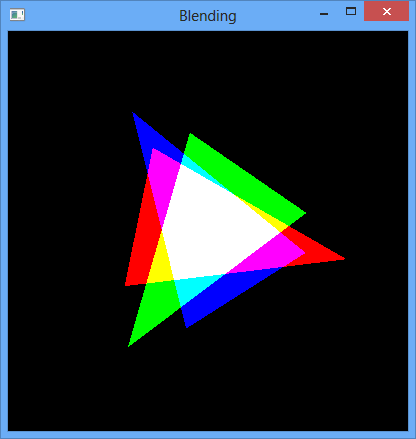
\includegraphics[width=0.5\textwidth]{blending.png}
\end{center}
\end{exercise}

\begin{exercise}{2}{0.5}
Besides alpha-transparency, blending can be used to achieve effects such as \emph{motion blur}, \emph{soft shadows} and \emph{depth of field}. In the second scene of the project (function \verb#draw_motionblur#), implement the motion blur effect for a horizontally moving triangle. To do that you essentially need to average several consecutive frames of triangle movement. Currently, the function renders 20 copies of the triangle, each shifted a bit to the right, one on top of the other. For the motion blur effect you have to configure blending so that each copy is multiplied by $1/20$ and added to whatever is currently on the screen. The result should look like the picture below.
\begin{center}
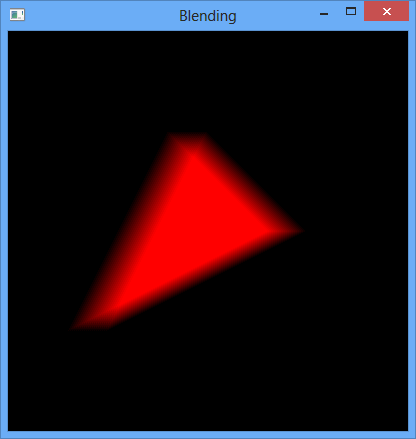
\includegraphics[width=0.5\textwidth]{motionblur.png}
\end{center}
\end{exercise}

\begin{exercise}{3*}{1}
The \emph{depth-of-field} effect aims to imitate the way real camera lenses work: objects located at around the \emph{focus distance} are sharp, and objects further away or closer than the focus distance are blurred. The effect can be implemented in a manner similar to motion blur. The only difference is that the average is not taken over moving frames, but over slightly jittered camera projections. Read about the approach in detail in Chapter 10 of the ``OpenGL Red Book''\footnote{\url{http://www.glprogramming.com/red/chapter10.html}} (or find other descriptions in the internet). Implement this effect on a simple scene with several objects at different distances from the camera. Use blending to implement it\footnote{Most (if not all) descriptions you will find in the internet will refer to the use of \emph{accumulation buffer} for averaging multiple frames. Accumulation buffer is, however, removed from the latest versions of OpenGL specification in favor of blending and pixel shaders. Hence, to keep up with the times, I require you to use blending in this exercise as well.}. An example image you may strive for is shown below. Notice how the green sphere is exactly at the focus distance. Also observe that the DOF is very small, so spheres even slightly out of focus look considerably blurred\footnote{This situation is actually typical for close-up photography and some people deliberately imitate small DOF in photos by blurring foreground and background to imitate miniature scenes. See \url{http://en.wikipedia.org/wiki/Tilt\%E2\%80\%93shift_photography}}.
\begin{center}
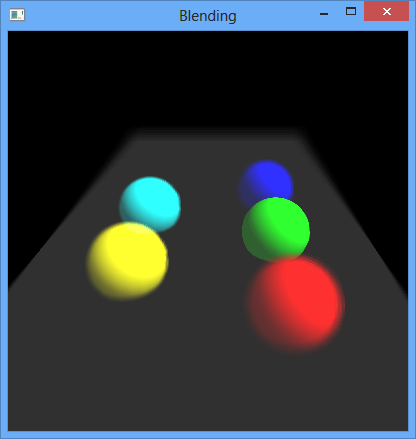
\includegraphics[width=0.5\textwidth]{dof.png}
\end{center}
\end{exercise}

Finally, note that blending is a general concept, not specific only to OpenGL. For example, the same notions apply to Allegro (see \verb#al_set_blender#). HTML5 provides limited blending support via \verb#globalCompositeOperation#.

\section{Depth Buffer}
In the lecture we learned about the \emph{Z-buffer} (a.k.a \emph{depth buffer}) algorithm. The simple take-away message was that you should always have it enabled when working with 3D graphics. Let us now practice the more explicit use of the depth buffer on an (admittedly somewhat artificial) example\footnote{Think how you could achieve the same effect without resorting to depth buffer manipulations}.

\begin{exercise}{4}{0.5}
Open the project \verb#2_DepthBuffer#. It contains a rendering of a model, that should be familiar to you from exercise session 4. Suppose we would like to render only the part of the model, that lies closer to the camera than distance 6 (which is the distance to the center of the model). Image below illustrates the desired effect.
\begin{center}
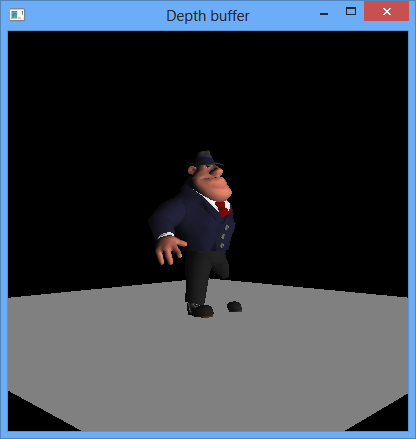
\includegraphics[width=0.5\textwidth]{halfmodel.png}
\end{center}

To achieve this effect using the depth buffer do the following:
\begin{enumerate}
\item Draw the floor rectangle (\verb#draw_floor#) as usual.
\item Switch off drawing to the screen using \texttt{glColorMask}. Now you will only render to the depth buffer.
\item Draw a large rectangle (e.g. $100\times 100$) perpendicular to the viewer and at distance $6$ from it. Hint: recall that in the camera frame the $z$ axis points straight out of the screen.
\item Switch drawing to the screen back on and render the model as usual.
\end{enumerate}

Implement this in \verb#2_DepthBuffer#.
\end{exercise}

\section{Stencil Buffer}
Another useful auxiliary buffer is the \emph{stencil buffer}. Like the depth buffer, it keeps a separate value for each pixel, however the values are integers. You can specify an operation used to update the stencil buffer using \texttt{glStencilOp}. 

For example, \verb#glStencilOp(GL_INCR, GL_INCR, GL_INCR)# specifies that the value in the stencil buffer has to be increased each time a pixel could be drawn to it. Hence, if you start with a zeroed stencil buffer and render the whole scene, each value in the stencil buffer will count how many triangles were rendered at that pixel.

In addition to the buffer update rule, you may specify a \emph{stencil test}, which lets you decide on a pixel-per-pixel basis, which pixels should be drawn, depending on their stencil values. You enable the stencil test using \\ \verb#glEnable(GL_STENCIL_TEST)# and specify the type of test using \verb#glStencilFunc#.

Stencil buffer allows to implement numerous interesting effects, such as shadows, reflections, contours or object intersections. Here we shall use it to implement a simple planar reflection.

\begin{exercise}{5}{1}
Open project \verb#3_StencilBuffer# and modify it as follows:
\begin{enumerate}
\item Modify \texttt{glutInitDisplayMode} to allocate memory for the stencil buffer. Add a line to enable the stencil test.
\item Modify \texttt{display} function to implement the following algorithm:
\begin{enumerate}
\item Clear the color, depth and stencil buffers
\item Render the floor \emph{only} to the stencil buffer (disable writing to depth or color buffers temporarily), setting stencil buffer values to $1$ for all pixels of the floor.
\item Set the stencil test to pass only for pixels that have stencil buffer value of $1$. Render the figure of a man, mirrored about the $y=0$ plane. Due to stenciling, only ``floor'' pixels will be affected.
\item Set the stencil test to always pass. Render the floor, using alpha-transparency with a coefficient of $0.8$ for the floor.
\item Finally, render the man standing on the floor as normal.
\end{enumerate}
\end{enumerate}
The result should look as follows.
\begin{center}
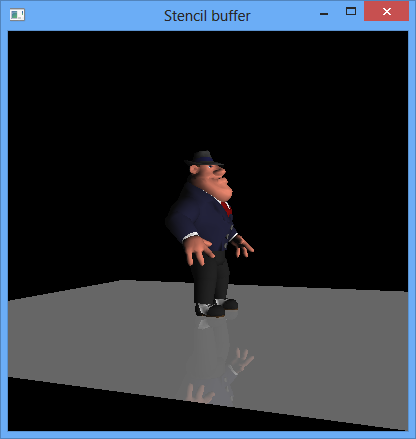
\includegraphics[width=0.6\textwidth]{stencil.png}
\end{center}

\end{exercise}

\end{document}
